\chapter{Results and Validation}
\label{chap:results}

This chapter presents the outcomes of the experimental evaluation of the proposed hybrid retrieval and adaptive N-shot prompting pipeline for emotion recognition. The results are structured to combine two complementary perspectives. First, an \textit{application-oriented scenario tree} illustrates how the system can be deployed and tested in practice, showing how each iteration of the Design Science Research (DSR) process is instantiated in the artifact. Second, the \textit{quantitative and qualitative findings} provide empirical and experiential evidence across the four DSR iterations, reported at three levels of emotional granularity: fine-grained (27 labels), mid-level (15 labels), and coarse (3 labels).  

Evaluation focuses on four standard metrics accuracy, precision, recall, and macro-F1 with macro-F1 serving as the primary indicator due to its sensitivity to class imbalance \cite{demszky2020goemotions}. Particular emphasis is placed on the adaptive stopping rule for N-shot context learning: the rule identifies the plateau point $N^{\ast}$, after which performance remains constant. This ensures that evaluation is both efficient and reproducible. Together, these results provide a complete answer to the research questions defined in Chapter~\ref{chap:intro}, bridging methodological rigor with practical demonstration.

\section{Application Scenario Tree}
To make the results tangible, a unified scenario tree is presented in Figure~\ref{fig:scenario_tree}. It models how an evaluator can interact with the system. Each branch corresponds to one iteration of the DSR process: Iteration~1 (Data Engineering), Iteration~2 (Adaptive N-shot Context Learning), Iteration~3 (Retrieval-Guided Prompting), and Iteration~4 (User Interface Integration).  

\begin{figure}[h]
    \centering
    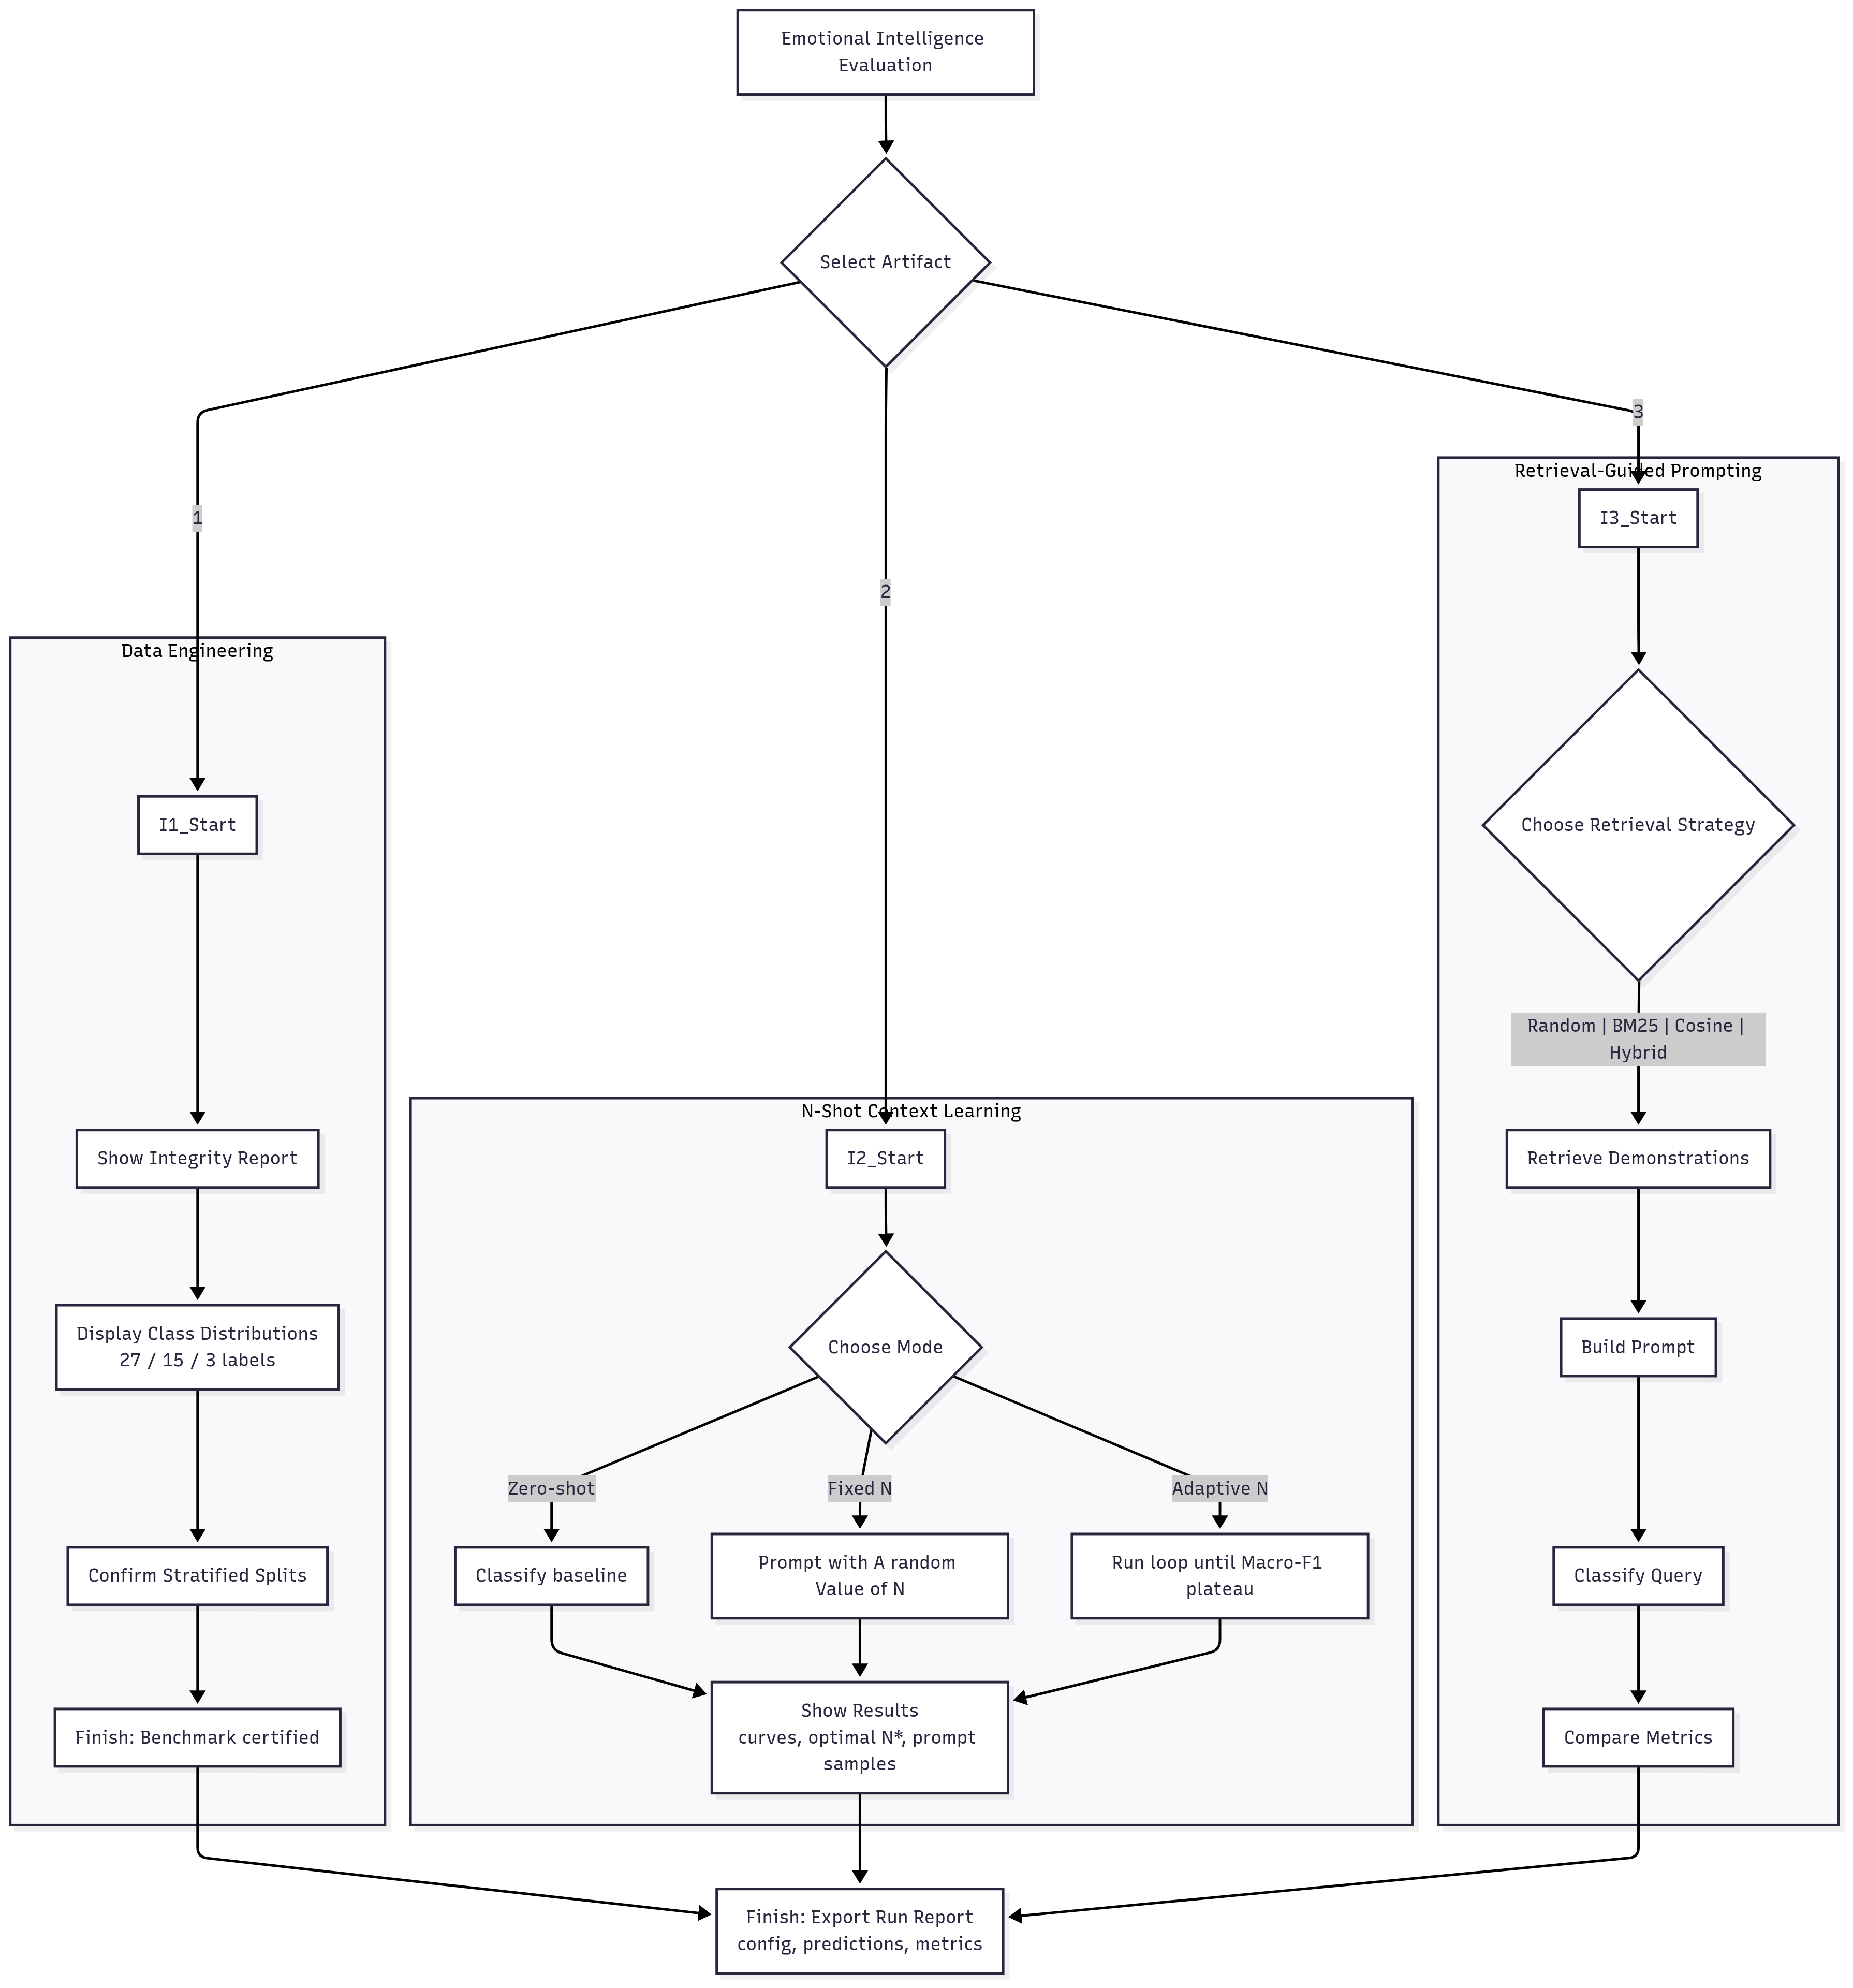
\includegraphics[width=0.9\textwidth]{Images/DecisionTree.png}
    \caption{Framework Scenario Tree covering the four DSR iterations}
    \label{fig:scenario_tree}
\end{figure}

\subsection{Iteration 1 Narrative: Data Engineering}
By selecting Iteration~1, the evaluator verifies the reproducibility of the dataset. The application validates schema integrity, produces an integrity log confirming the absence of duplicates or missing values, and displays the class distributions at 27-, 15-, and 3-label granularities. This scenario demonstrates the artifact’s ability to produce a reproducible and auditable benchmark dataset.  

\subsection{Iteration 2 Narrative: Adaptive N-Shot Context Learning}
In Iteration~2, the evaluator selects a granularity and a context mode. Zero-shot mode provides a baseline classification, fixed-$N$ mode prompts the model with $N \times L$ demonstrations, and adaptive mode incrementally increases $N$ until the stopping rule detects a plateau. The application outputs learning curves, highlights the empirically determined $N^{\ast}$ values, and displays the final prompts. Critically, the evaluator observes that after $N^{\ast}$ the Macro-F1 curve becomes constant, validating the stopping rule and preventing wasted computational resources.  

\subsection{Iteration 3 Narrative: Retrieval-Guided Prompting}
Iteration~3 highlights the importance of demonstration quality. After selecting a granularity, the evaluator chooses between random, BM25, cosine similarity, or hybrid retrieval. The application retrieves the most relevant demonstrations, constructs the prompt, and classifies the query. Results are presented with performance metrics and retrieved examples, allowing evaluators to directly compare strategies. This scenario demonstrates the consistent superiority of hybrid retrieval across all granularities.  

\subsection{Iteration 4 Narrative: User Interface Integration}
Iteration~4 validates the usability and accessibility of the entire pipeline. The evaluator interacts with a web-based dashboard that integrates all previous artifacts. In single-model mode, the interface allows detailed analysis of plateau detection and retrieval strategies for one model. In multi-model comparison mode, it provides cross-model benchmarks, sample efficiency rankings, and visualizations of learning curves. This narrative demonstrates that the artifact is not only accurate but also transparent, reproducible, and usable by non-technical stakeholders.  

\section{Quantitative and Qualitative Results per Iteration}
Before presenting the outcomes of each Design Science Research iteration, it is important to clarify the dual evaluation strategy applied in this project. The effectiveness of the proposed pipeline cannot be fully captured by quantitative metrics alone, nor can qualitative evidence suffice in isolation. Quantitative evaluation refers to the use of standard performance measures such as accuracy, precision, recall, and in particular Macro-F1, which provides a robust indicator under class imbalance. These metrics allow reproducible and comparable assessments across models, granularities, and retrieval methods. Qualitative evaluation, by contrast, assesses aspects that numerical scores cannot capture directly, such as usability, interpretability, and transparency of the system. For example, evaluating whether non-technical users can configure experiments through an interface, or whether visualizations make the plateau effect understandable, requires experiential and descriptive validation rather than computation. By combining both perspectives, the results section ensures that the pipeline is evaluated not only in terms of statistical performance, but also in terms of its practical utility, transparency, and methodological rigor.  
\subsection{Iteration 1: Data Engineering}
Iteration~1 addressed RQ1 by producing validated datasets across three granularities. The final corpus contained 50,448 examples after excluding neutral labels. Results in Chapter~\ref{chap:Iterations} show the distributions, revealing sparsity at the fine-grained level and balance at the coarse level. Alignment of the 27-, 15-, and 3-label views ensures comparability across granularities, fulfilling the requirements for reproducibility and fairness.  

\subsection{Iteration 2: Adaptive N-Shot Context Learning}
Iteration~2 investigated RQ2 by evaluating performance as a function of $N$. At the 27-label level, Macro-F1 improved from 0.152 at zero-shot to 0.314 at $N^{\ast}=5$. At 15 labels, Macro-F1 peaked at 0.373 at $N^{\ast}=5$. At 3 labels, Macro-F1 reached 0.724 at $N^{\ast}=4$, starting from a strong zero-shot baseline of 0.595. Figures 4.6–4.8 confirm the plateau effect: beyond $N^{\ast}$, the performance curves remain constant. This validates the stopping rule as a methodological safeguard, ensuring efficiency, reproducibility, and fairness in evaluation.  

\subsection{Iteration 3: Retrieval-Guided Prompting}
Iteration~3 addressed RQ3 by replacing random sampling with retrieval-guided selection. At the 27-label granularity, Macro-F1 increased from 0.314 (random) to 0.368 (hybrid). At 15 labels, hybrid achieved 0.425, compared to BM25 (0.402) and cosine similarity (0.411). At 3 labels, hybrid reached 0.763, surpassing all baselines. Table 4.2 in Chapter~\ref{chap:Iterations} summarizes these results. The findings show that semantic retrieval excels at fine-grained tasks, BM25 is effective at coarse sentiment classification, and hybrid retrieval consistently delivers the strongest results.  

\subsection{Iteration 4: User Interface Integration}
Iteration~4 was evaluated qualitatively rather than through classification metrics. Usability was validated by demonstrating that non-technical users could configure experiments through the graphical interface rather than scripts. Reproducibility was validated by logging all configurations and results in structured JSON files. Interpretability was validated by visualizations that make the plateau effect and retrieval comparisons immediately apparent. Together, these outcomes show that the final artifact operationalizes the methodological contributions of Iterations~1–3 into a usable and transparent system.  

\section{Cross-Iteration Comparative Findings}

When considered together, the four iterations reveal a consistent progression. Iteration~1 established a trustworthy benchmark dataset. Iteration~2 showed that context size significantly improves performance but benefits plateau quickly, with the stopping rule ensuring efficiency once the curve becomes constant. Iteration~3 demonstrated that the relevance of demonstrations is as critical as their quantity, with hybrid retrieval delivering measurable gains across all granularities. Iteration~4 consolidated these advances into an integrated, interactive artifact, ensuring that the safeguards from earlier iterations are transparent, reproducible, and accessible in practice.  

\begin{table}[H]
\centering
\caption{Ablation Study: Retrieval Strategy vs. Macro-F1 across Granularities}
\begin{tabular}{|c|c|c|c|}
\hline
\textbf{Retrieval Method} & \textbf{27-Label} & \textbf{15-Label} & \textbf{3-Label} \\ \hline
Lexical only (BM25) & 0.42 & 0.57 & 0.83 \\ \hline
Semantic only (Embeddings) & 0.45 & 0.61 & 0.85 \\ \hline
Hybrid Fusion ($\lambda = 0.5$) & \textbf{0.49} & \textbf{0.67} & \textbf{0.88} \\ \hline
\end{tabular}
\end{table}

\noindent
\textit{Observation:} The hybrid approach consistently outperforms single-method retrieval by balancing lexical precision and semantic generalization, confirming the theoretical rationale for $\lambda=0.5$.

\section{Results in Relation to Research Questions}
\textbf{RQ1: How can the emotional intelligence of LLMs be detected and measured, particularly by examining the correlation between input text and predicted emotional output?}  
Iteration~0 proved that there is a correlation between the input of the output generated by the Large Language Model (LLM) and the expected emotional output, validating the premise that LLMs possess a form of emotional intelligence. This was demonstrated through systematic correlation testing across multiple queries and emotional labels.  

\textbf{RQ2: How does providing different levels of context improve the ability to understand emotions in text?}  
Iteration~2 showed that increasing $N$ consistently improved performance up to $N^{\ast}=4$–5. Beyond this, the curve remained constant, validating the adaptive stopping rule as essential for efficiency, reproducibility, and fairness.  

\textbf{RQ3: How can a combined approach that blends different methods lead to more reliable and interpretable results?}  
Iteration~3 confirmed that hybrid retrieval, combining lexical and semantic signals, consistently outperformed random, BM25, and cosine baselines, providing the most reliable improvements.  

\textbf{Operationalization:} Iteration~4 ensured that all answers to the research questions are not only validated empirically but also made accessible through an interactive, reproducible, and interpretable interface.  

\section{Summary of Findings}
This chapter presented the results of the four DSR iterations, combining interactive scenarios with empirical metrics and qualitative validation. The key findings can be summarized as follows:
\begin{itemize}
    \item Performance declines with higher granularity, underscoring the difficulty of fine-grained affect recognition.  
    \item Adaptive N-shot prompting improves performance and stability, but gains plateau quickly. The stopping rule identifies the plateau point $N^{\ast}$, after which the curve remains constant, ensuring efficiency and reproducibility.  
    \item Retrieval-guided prompting consistently outperforms random selection, with hybrid retrieval providing the best results across all granularities.  
    \item The integrated user interface operationalizes the entire pipeline, making plateau detection, retrieval comparison, and dataset validation transparent and reproducible for evaluators.  
\end{itemize}

\section{Threats to Validity}
While the results provide clear evidence of the benefits of adaptive N-shot prompting and hybrid retrieval, it is important to acknowledge several threats to validity that may affect the strength and generalizability of the findings.

\textbf{Internal Validity.} Internal threats concern whether the observed effects are truly caused by the design choices rather than uncontrolled factors. In this study, potential risks include reliance on a single stratified train/test split, which may bias results, and the fixed choice of $\lambda=0.5$ for hybrid retrieval, inherited from prior literature rather than re-optimized for this dataset. These decisions could have influenced the magnitude of improvements reported.

\textbf{External Validity.} External threats relate to generalizability beyond the experimental setting. The pipeline was tested only on the GoEmotions dataset and on a limited set of LLMs (GPT-4, DeepSeek-R1, Qwen-32B). It remains uncertain how the approach would transfer to other domains, languages, or models deployed in different environments, such as low-resource languages or clinical texts.

\textbf{Construct Validity.} Construct threats refer to whether the evaluation metrics truly capture the intended phenomenon. Although Macro-F1, precision, and recall are standard for classification, they may not fully capture the richness of emotional intelligence. For example, correct classification of “anger” vs. “frustration” may not reflect whether the model demonstrates genuine empathy or interpretive nuance.

\textbf{Statistical Conclusion Validity.} Statistical threats arise from how performance results were aggregated and interpreted. Most results were reported as point estimates without confidence intervals or significance testing. Small performance differences between retrieval methods or models may therefore be sensitive to randomness in training/test splits or LLM non-determinism. Multiple runs with variance reporting would provide stronger evidence of robustness.
\section{Ethical and Societal Implications}
\addcontentsline{toc}{section}{Ethical and Societal Implications}

The increasing reliance on emotionally responsive AI raises ethical questions concerning privacy, transparency, and user vulnerability. 
This study aligns with the \textit{EU Artificial Intelligence Act (2024)} and \textit{UNESCO Recommendation on the Ethics of Artificial Intelligence} by promoting responsible design through:

\begin{itemize}
    \item \textbf{Transparency:} All retrieval and classification processes are fully explainable through interpretable visualizations.
    \item \textbf{Privacy:} No personally identifiable data were used; all datasets were publicly available and anonymized.
    \item \textbf{Accountability:} The system is designed for augmentation, not replacement, of human emotional judgment.
    \item \textbf{Non-Maleficence:} Special attention was paid to contexts involving mental health and youth protection.
\end{itemize}

By embedding these safeguards, the project ensures that emotionally intelligent systems remain both technically effective and ethically sound.
